\documentclass{article}

\usepackage{tikz}

 

\begin{document}

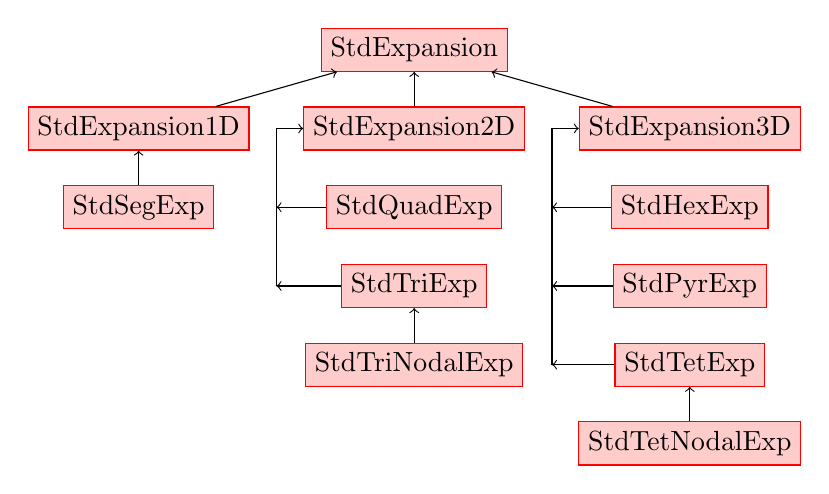
\begin{tikzpicture}[outline/.style={draw=#1,fill=#1!20}]

%NODES


\node [outline=red] (StdExpansion)                                   at (3.5,0)          {StdExpansion};

\node [outline=red] (StdExpansion1D)                              at (0,-1)        {StdExpansion1D};
\node [outline=red] (StdExpansion2D)                              at (3.5,-1)        {StdExpansion2D};
\node [outline=red] (StdExpansion3D)                              at (7,-1)        {StdExpansion3D};

\node [outline=red] (StdSegExp)                    at (0,-2)         {StdSegExp};
\node [outline=red] (StdQuadExp)                    at (3.5,-2)         {StdQuadExp};
\node [outline=red] (StdTriExp)                    at (3.5,-3)         {StdTriExp};
\node [outline=red] (StdTetExp)                    at (7,-4)         {StdTetExp};
\node [outline=red] (StdPyrExp)                    at (7,-3)         {StdPyrExp};
\node [outline=red] (StdHexExp)                    at (7,-2)         {StdHexExp};

\node [outline=red] (StdTriNodalExp)                    at (3.5,-4)         {StdTriNodalExp};
\node [outline=red] (StdTetNodalExp)                    at (7,-5)         {StdTetNodalExp};

%CONNECTIONS


\draw[<-] (StdExpansion2D)--(1.75,-1);

\draw (1.75,-2) -- (1.75,-1) ;
\draw[<-] (1.75,-2)--(StdQuadExp);

\draw (1.75,-3) -- (1.75,-2) ;
\draw[<-] (1.75,-3)--(StdTriExp);

\draw[<-] (StdExpansion3D)--(5.25,-1);

\draw (5.25,-2) -- (5.25,-1) ;
\draw[<-] (5.25,-2)--(StdHexExp);

\draw (5.25,-3) -- (5.25,-2) ;
\draw[<-] (5.25,-3)--(StdPyrExp);

\draw (5.25,-4) -- (5.25,-3) ;
\draw[<-] (5.25,-4)--(StdTetExp);

%\draw[->] (8,-4)--(8,0);
%\draw[->](ExpListHomogeneous1D)--(8,-4);

\path[<-]  (StdExpansion)      edge (StdExpansion1D)
                 (StdExpansion)      edge (StdExpansion2D)
                 (StdExpansion)      edge (StdExpansion3D)
                 (StdExpansion1D)      edge (StdSegExp)
                 (StdTetExp) edge  (StdTetNodalExp)
                 (StdTriExp) edge (StdTriNodalExp);

\end{tikzpicture}


\end{document}